%======================================================================
% CAPITULO 5: VISOR DE DOCUMENTOS SEGURO
%======================================================================

\chapter{Visor de Documentos Seguro}
\label{ch:visor}

Una de las caracteristicas exclusivas de \sdc{} es el \textbf{Visor Seguro}, que permite visualizar documentos confidenciales sin dejar rastro fisico en el disco duro.

\section{Visor Seguro de SDC}
\label{sec:visor-seguro}

El visor implementa un modelo de seguridad unico: los documentos se desencriptan directamente en la memoria RAM y nunca se escriben en el almacenamiento persistente.

\begin{figure}[H]
\centering
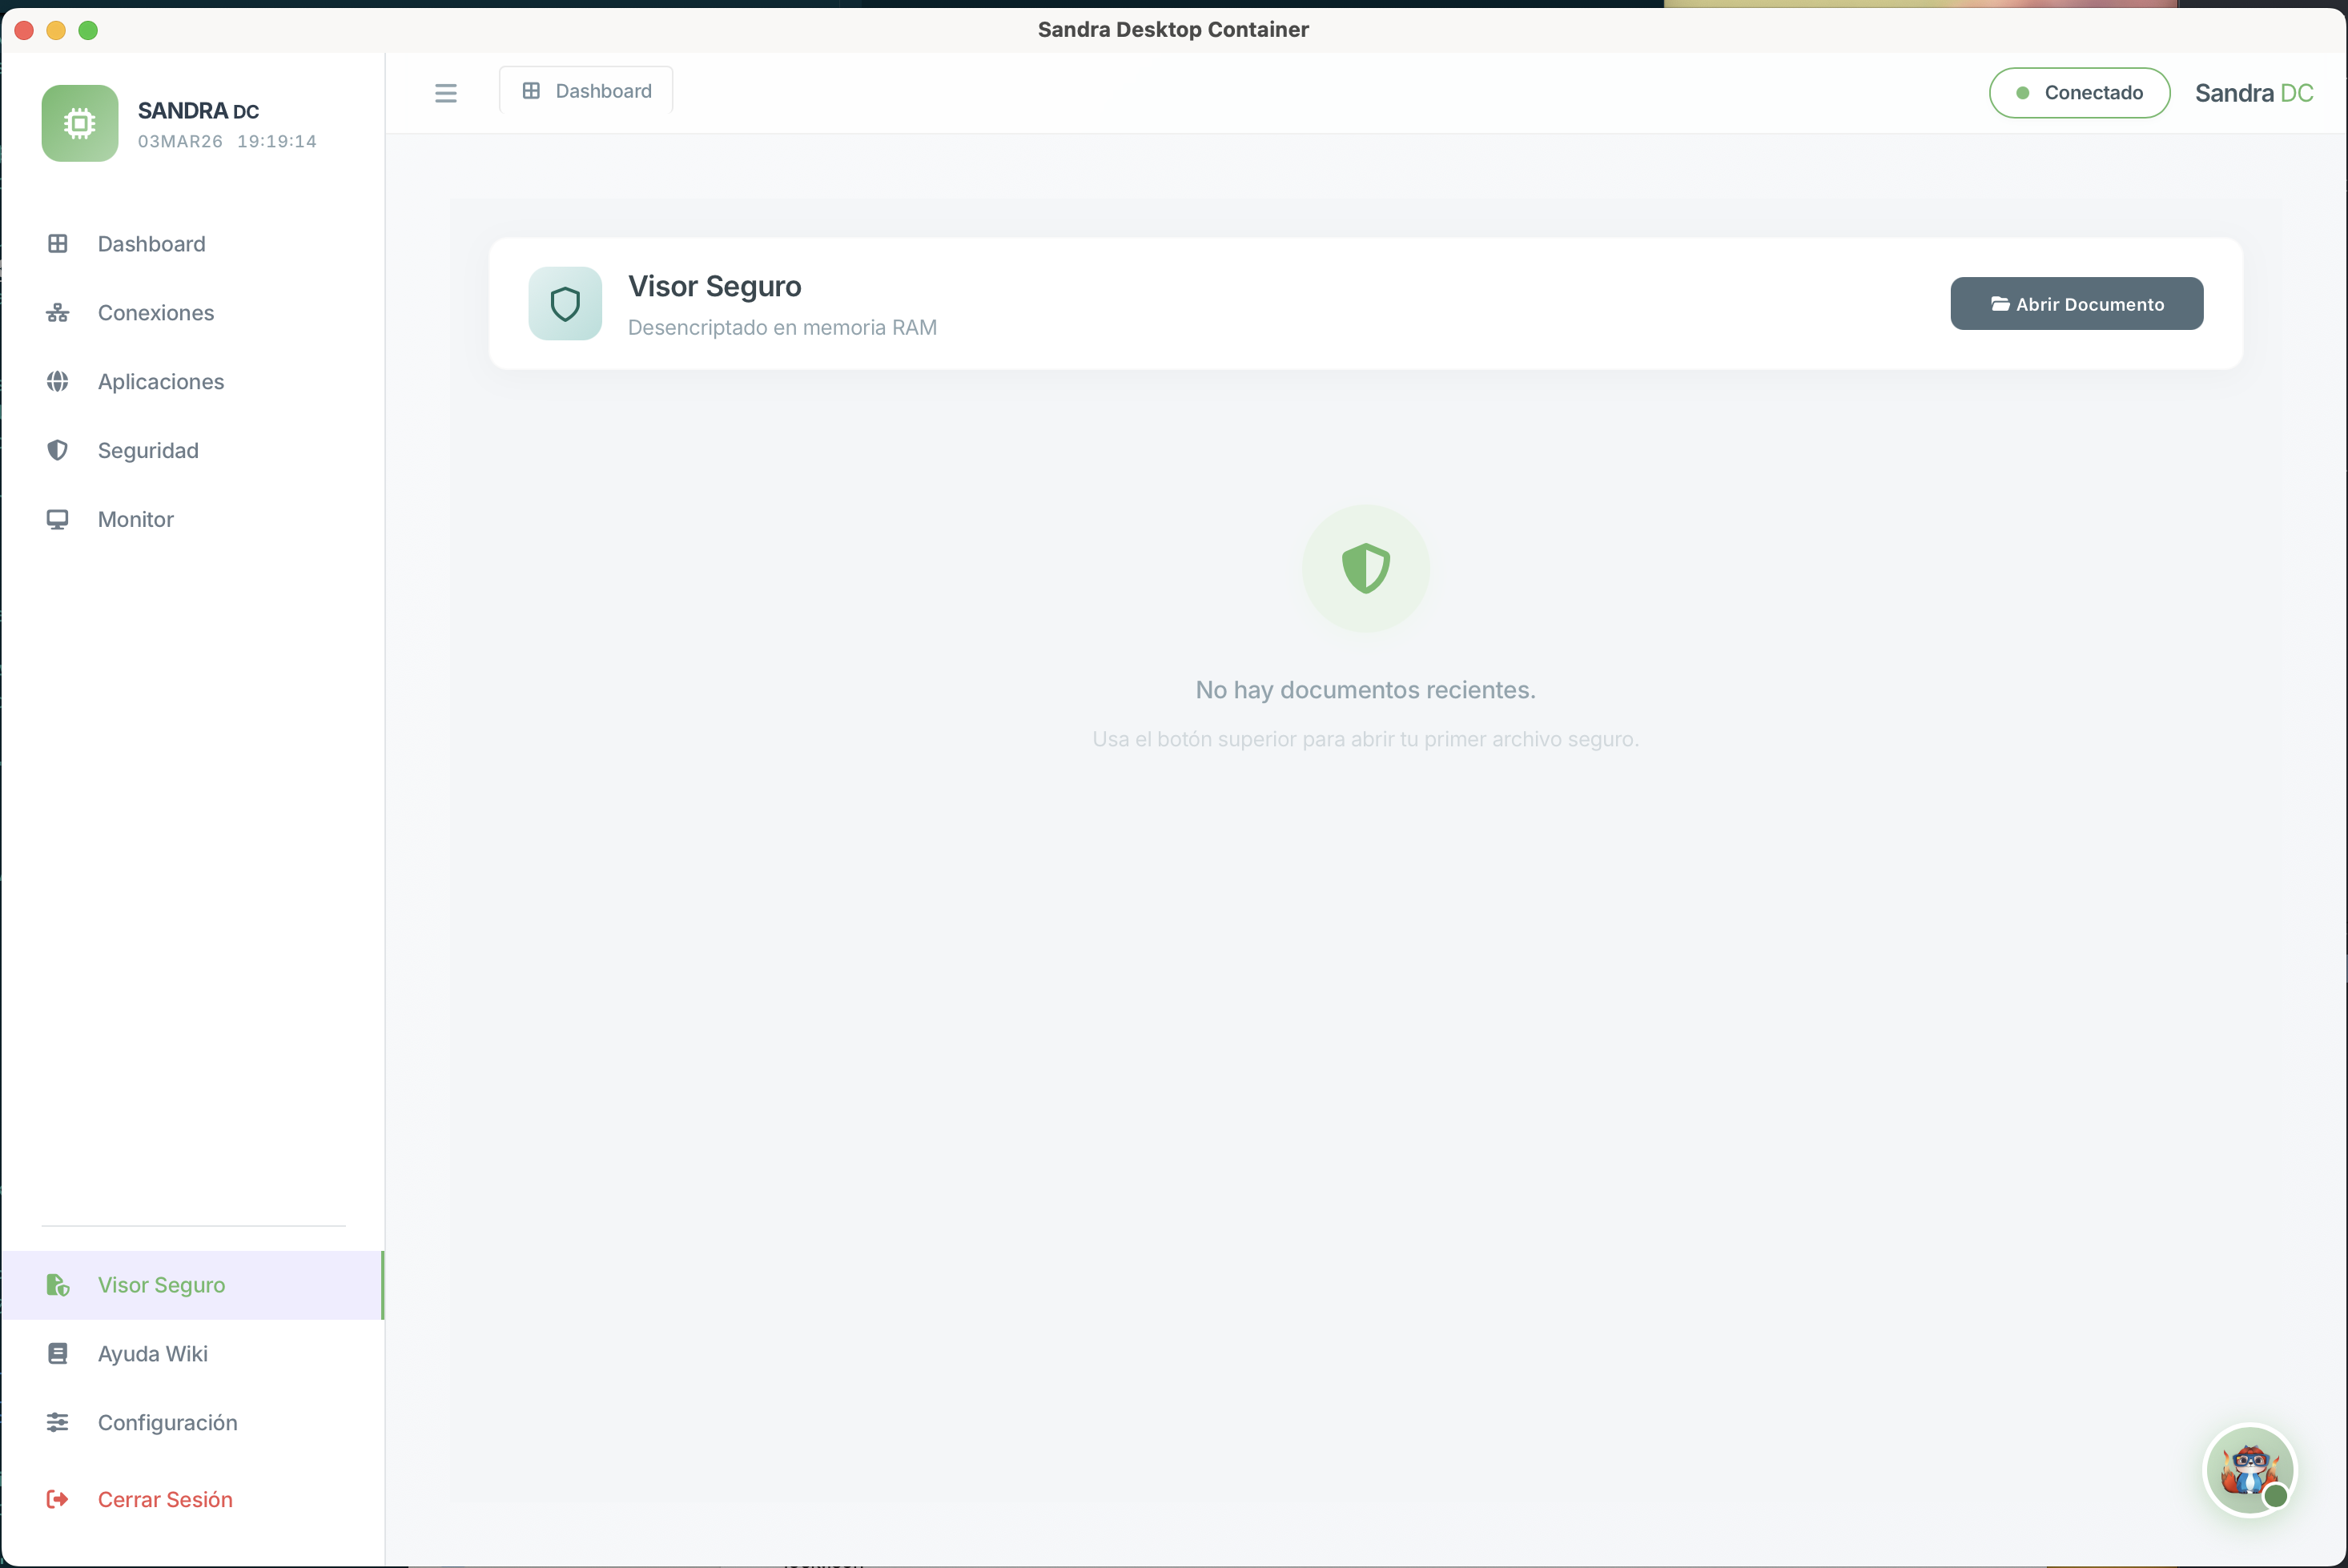
\includegraphics[width=0.95\textwidth]{anexos/11 visor.png}
\caption{Visor seguro de documentos}
\label{fig:visor}
\end{figure}

\subsection{Principio de Operacion}

\begin{enumerate}[leftmargin=*]
    \item El documento encriptado se transfiere desde el servidor origen
    \item Se descifra en tiempo real usando la clave privada del Client ID
    \item El contenido plano se mantiene unicamente en buffers de memoria RAM
    \item Se renderiza en el visor sin crear archivos temporales
    \item Al cerrar, los buffers se sobrescriben con ceros (zero-fill)
\end{enumerate}

\begin{quote}
\textbf{Proteccion Forense}\\
Al cerrar el visor, no queda rastro fisico del archivo en el disco duro. Esto evita la fuga de datos mediante tecnicas de analisis forense digital.
\end{quote}

\section{Formatos Soportados}
\label{sec:formatos}

El visor soporta multiples formatos de documento:

\begin{table}[H]
\centering
\begin{tabular}{p{4cm}p{3cm}p{6cm}}
\toprule
\textbf{Formato} & \textbf{Extension} & \textbf{Caracteristicas} \\
\midrule
PDF & .pdf & Visualizacion nativa con anotaciones \\
\midrule
Imagenes & .png, .jpg, .gif & Zoom, rotacion, filtros \\
\midrule
Documentos Office & .docx, .xlsx & Renderizado simplificado \\
\midrule
Texto Plano & .txt, .md, .json & Sintaxis resaltada \\
\midrule
Codigo Fuente & .rs, .ts, .js & Coloreado por lenguaje \\
\bottomrule
\end{tabular}
\caption{Formatos de documento soportados por el visor}
\label{tab:formatos}
\end{table}

\section{Lista de Documentos}
\label{sec:lista-documentos}

El panel de lista muestra todos los documentos disponibles.

\begin{figure}[H]
\centering
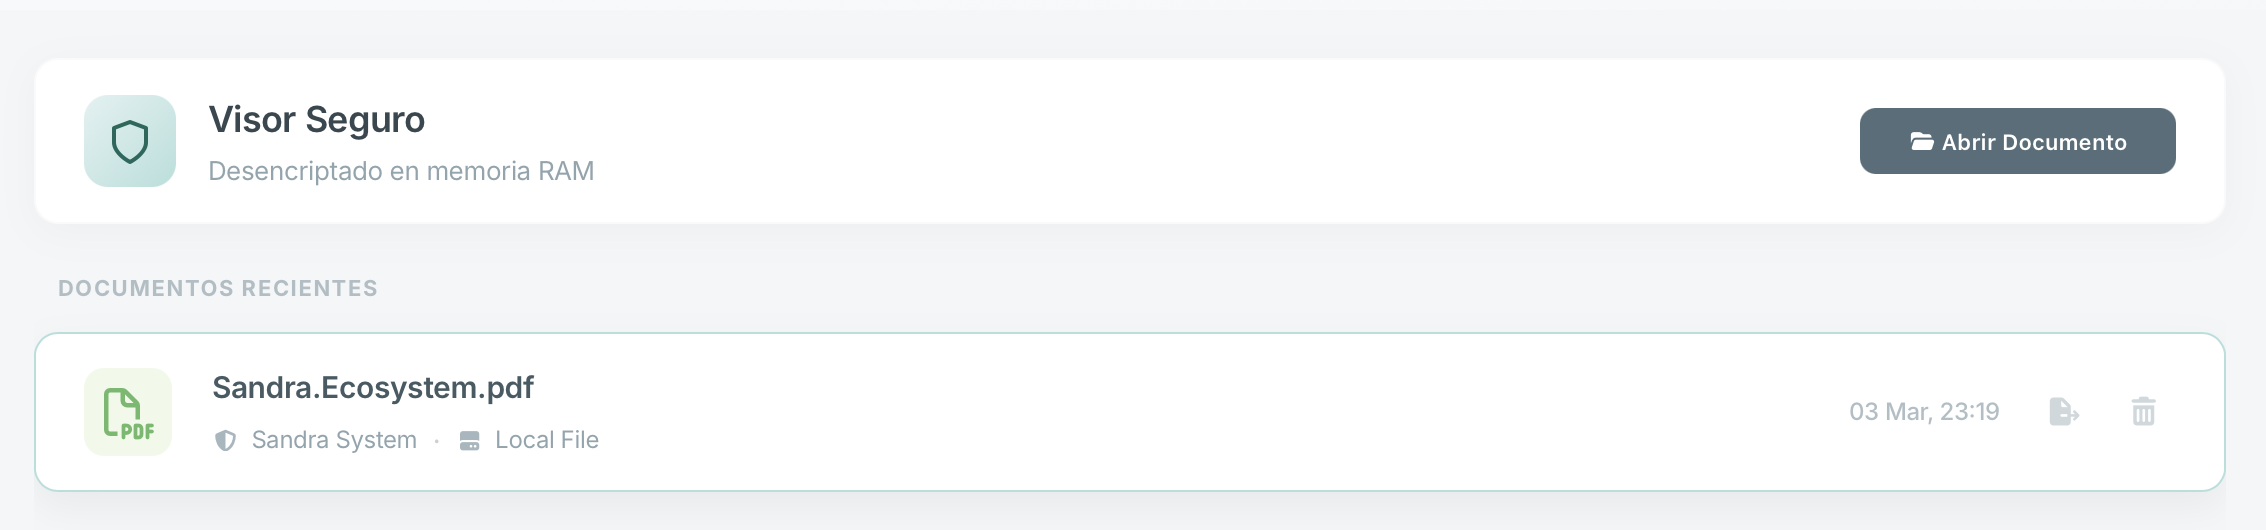
\includegraphics[width=0.95\textwidth]{anexos/13 visor list.png}
\caption{Lista de documentos en el visor}
\label{fig:visor-lista}
\end{figure}

\subsection{Informacion Visualizada}

Para cada documento se muestra:

\begin{itemize}[leftmargin=*]
    \item Nombre del archivo
    \item Tamanio en formato legible
    \item Fecha de ultima modificacion
    \item Estado de encriptacion (Verde: Encriptado)
    \item Propietario o autor
    \item Etiquetas de clasificacion
\end{itemize}

\section{Encriptacion de Documentos}
\label{sec:encriptacion}

\begin{figure}[H]
\centering
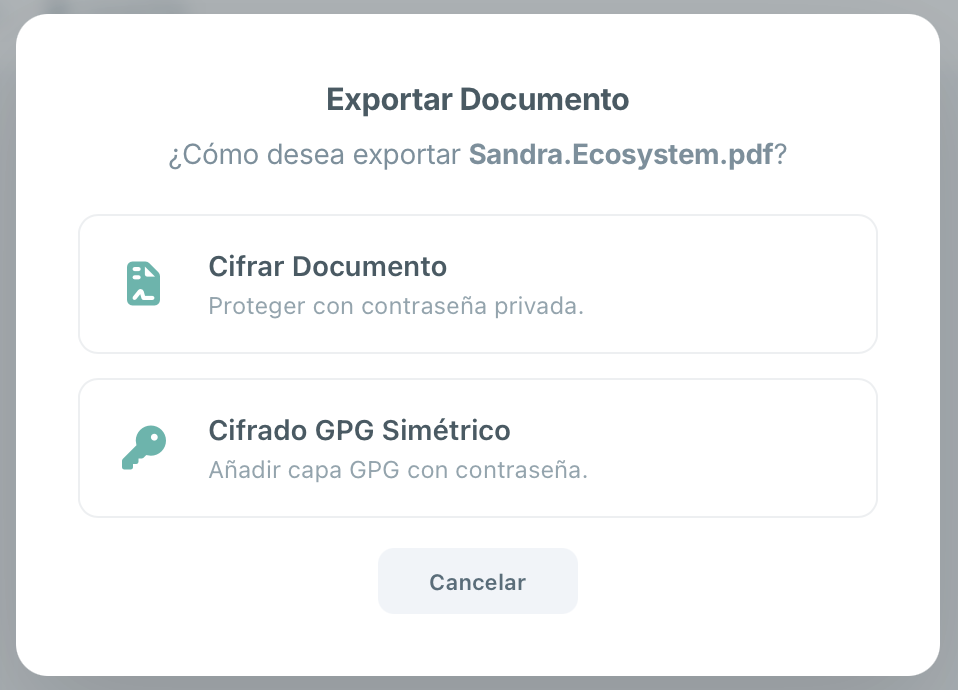
\includegraphics[width=0.95\textwidth]{anexos/14 visor encriptado.png}
\caption{Estado de documento encriptado}
\label{fig:visor-encriptado}
\end{figure}

\subsection{Esquema de Encriptacion}

SDC utiliza SSE (Sandra Secure Encryption), un esquema hibrido:

\begin{enumerate}
    \item \textbf{Cifrado Simetrico}: AES-256-GCM para el contenido
    \item \textbf{Cifrado Asimetrico}: RSA-4096 para proteger la clave AES
    \item \textbf{Clave de Sesion}: Generada aleatoriamente para cada documento
    \item \textbf{Derivacion}: HKDF-SHA256 para claves derivadas
\end{enumerate}

\subsection{Proceso de Cifrado}

\begin{enumerate}[leftmargin=*]
    \item Generar clave AES-256 aleatoria (32 bytes)
    \item Cifrar el documento con AES-256-GCM
    \item Cifrar la clave AES con la clave publica RSA del destinatario
    \item Empaquetar: documento cifrado + clave cifrada + metadatos
    \item Firmar digitalmente el paquete con la clave privada del emisor
\end{enumerate}

\section{Previsualizacion de Archivos}
\label{sec:preview}

El modo de previsualizacion permite obtener una vista rapida sin cargar el documento completo.

\begin{figure}[H]
\centering
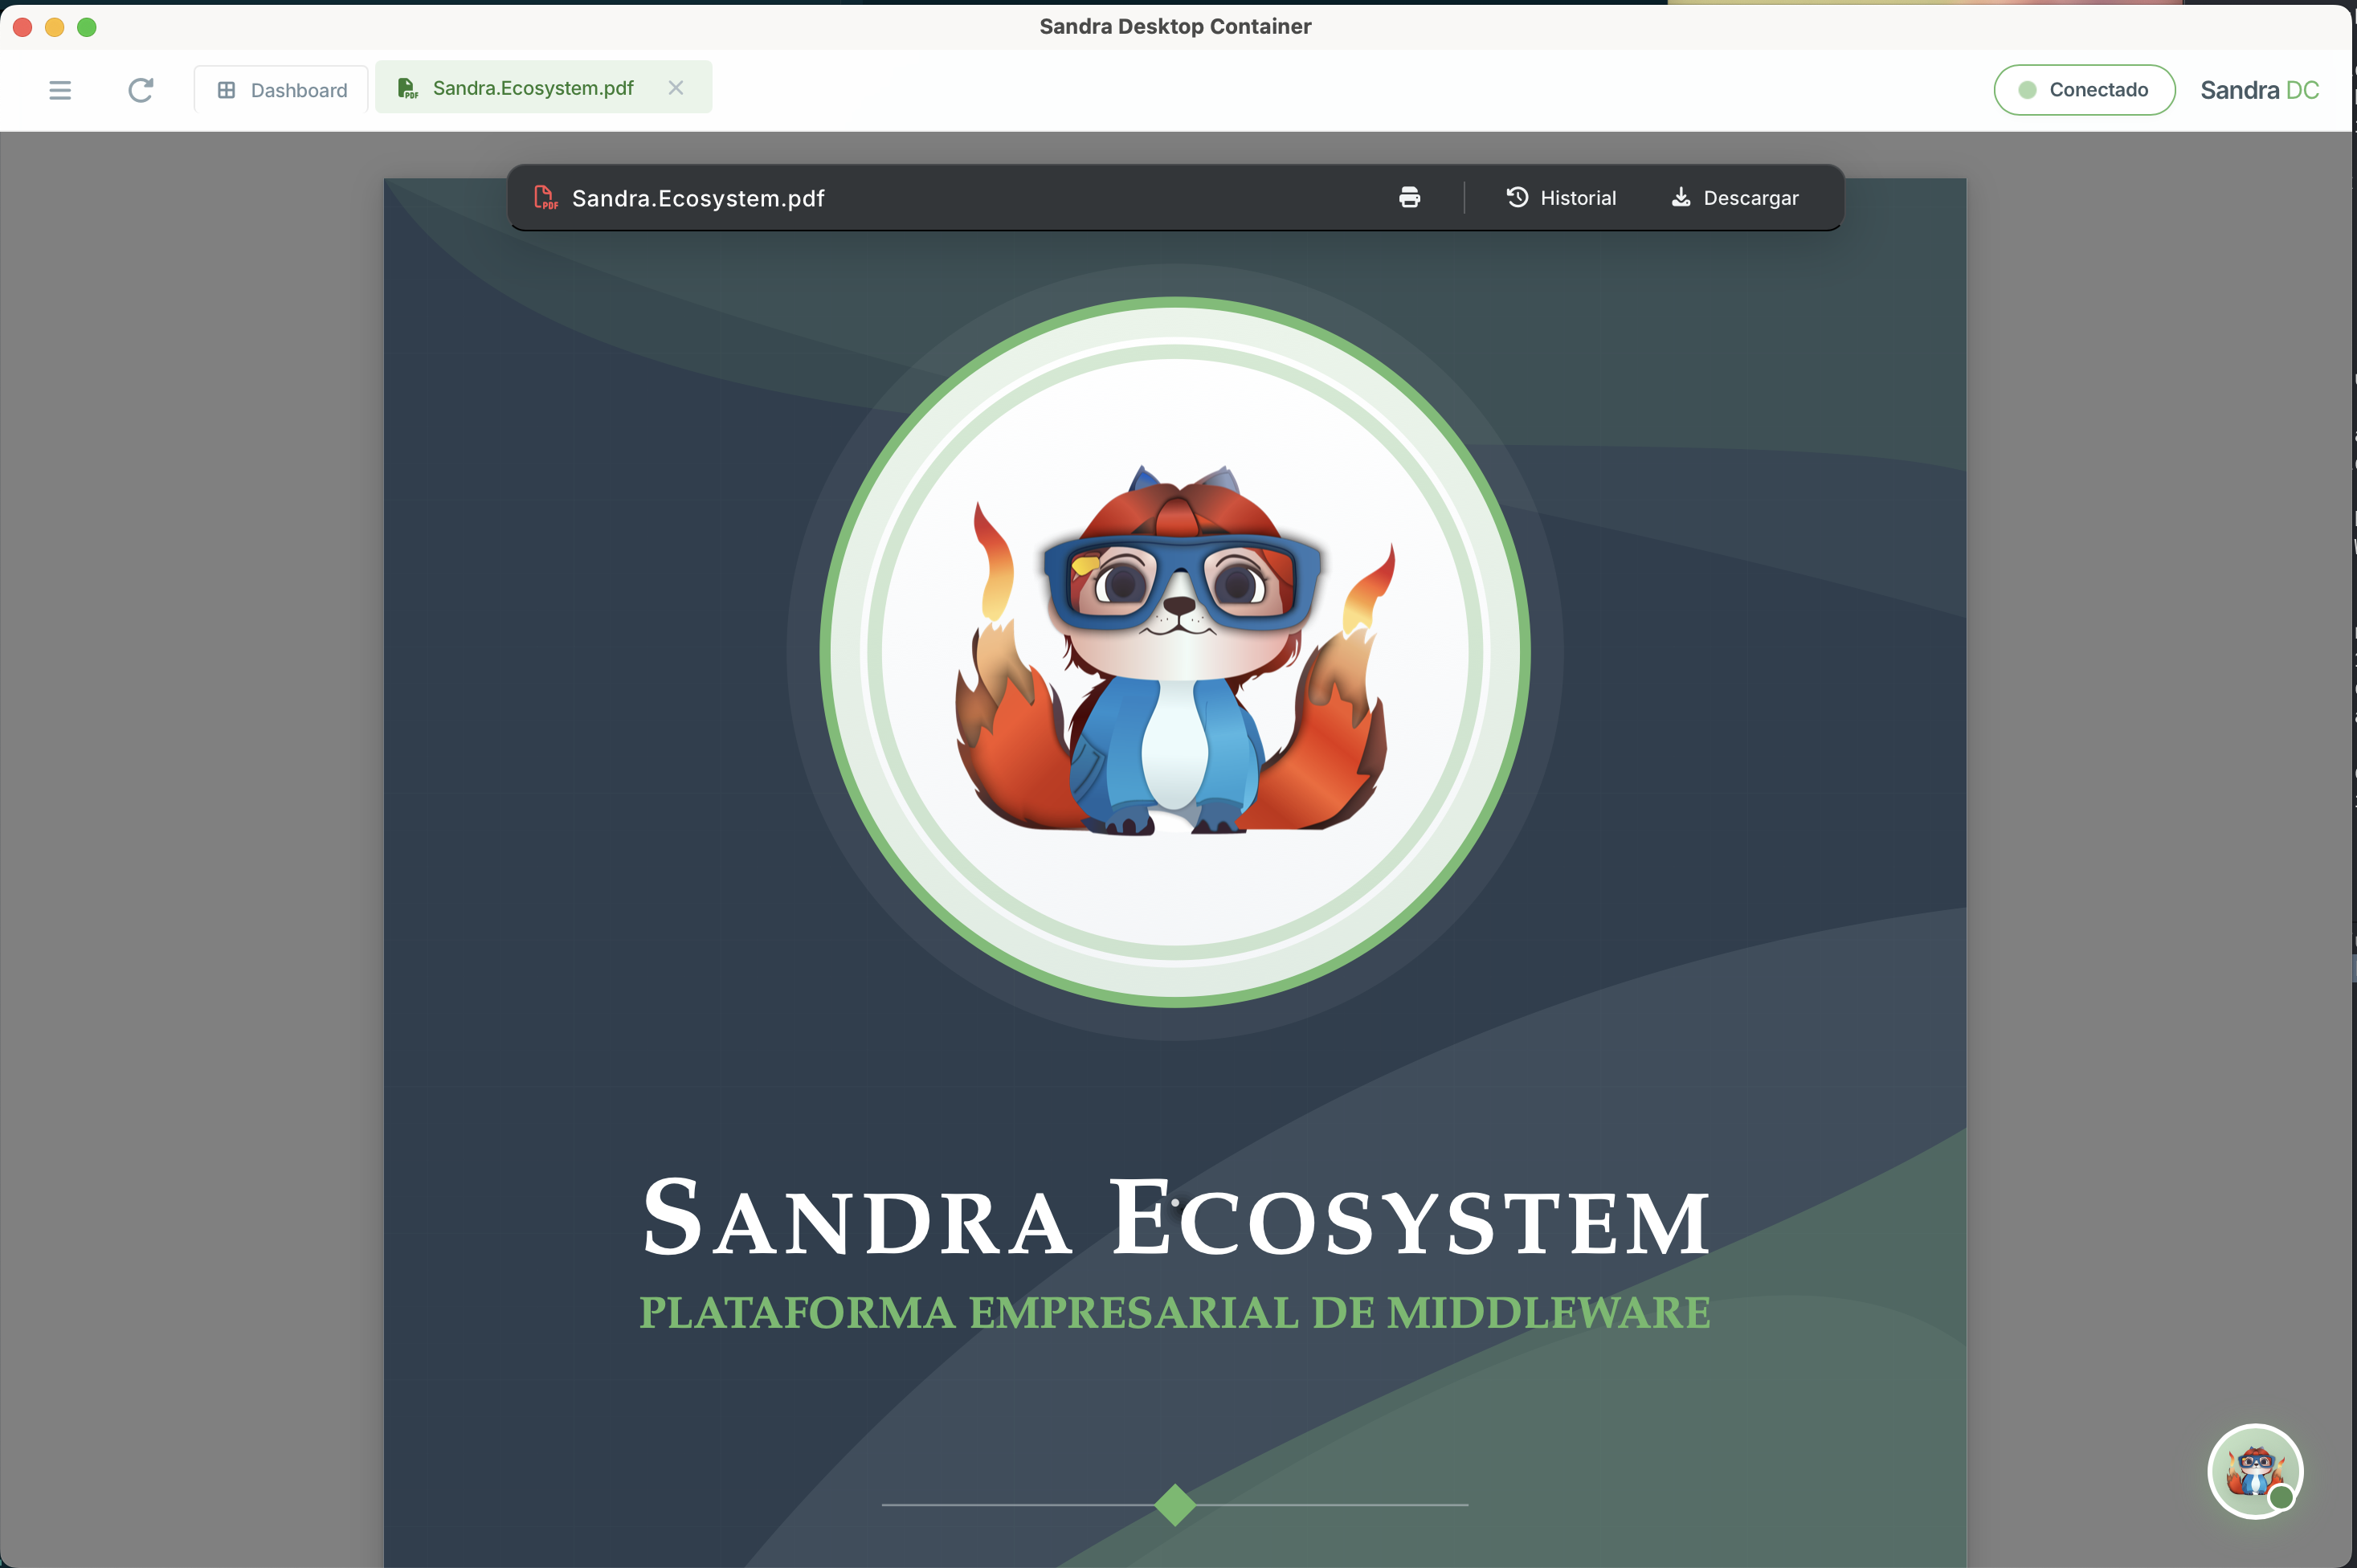
\includegraphics[width=0.95\textwidth]{anexos/12 preview-file.png}
\caption{Previsualizacion de archivo}
\label{fig:preview}
\end{figure}

\section{Configurador del Visor}
\label{sec:configurador}

El configurador permite ajustar el comportamiento del visor.

\begin{figure}[H]
\centering
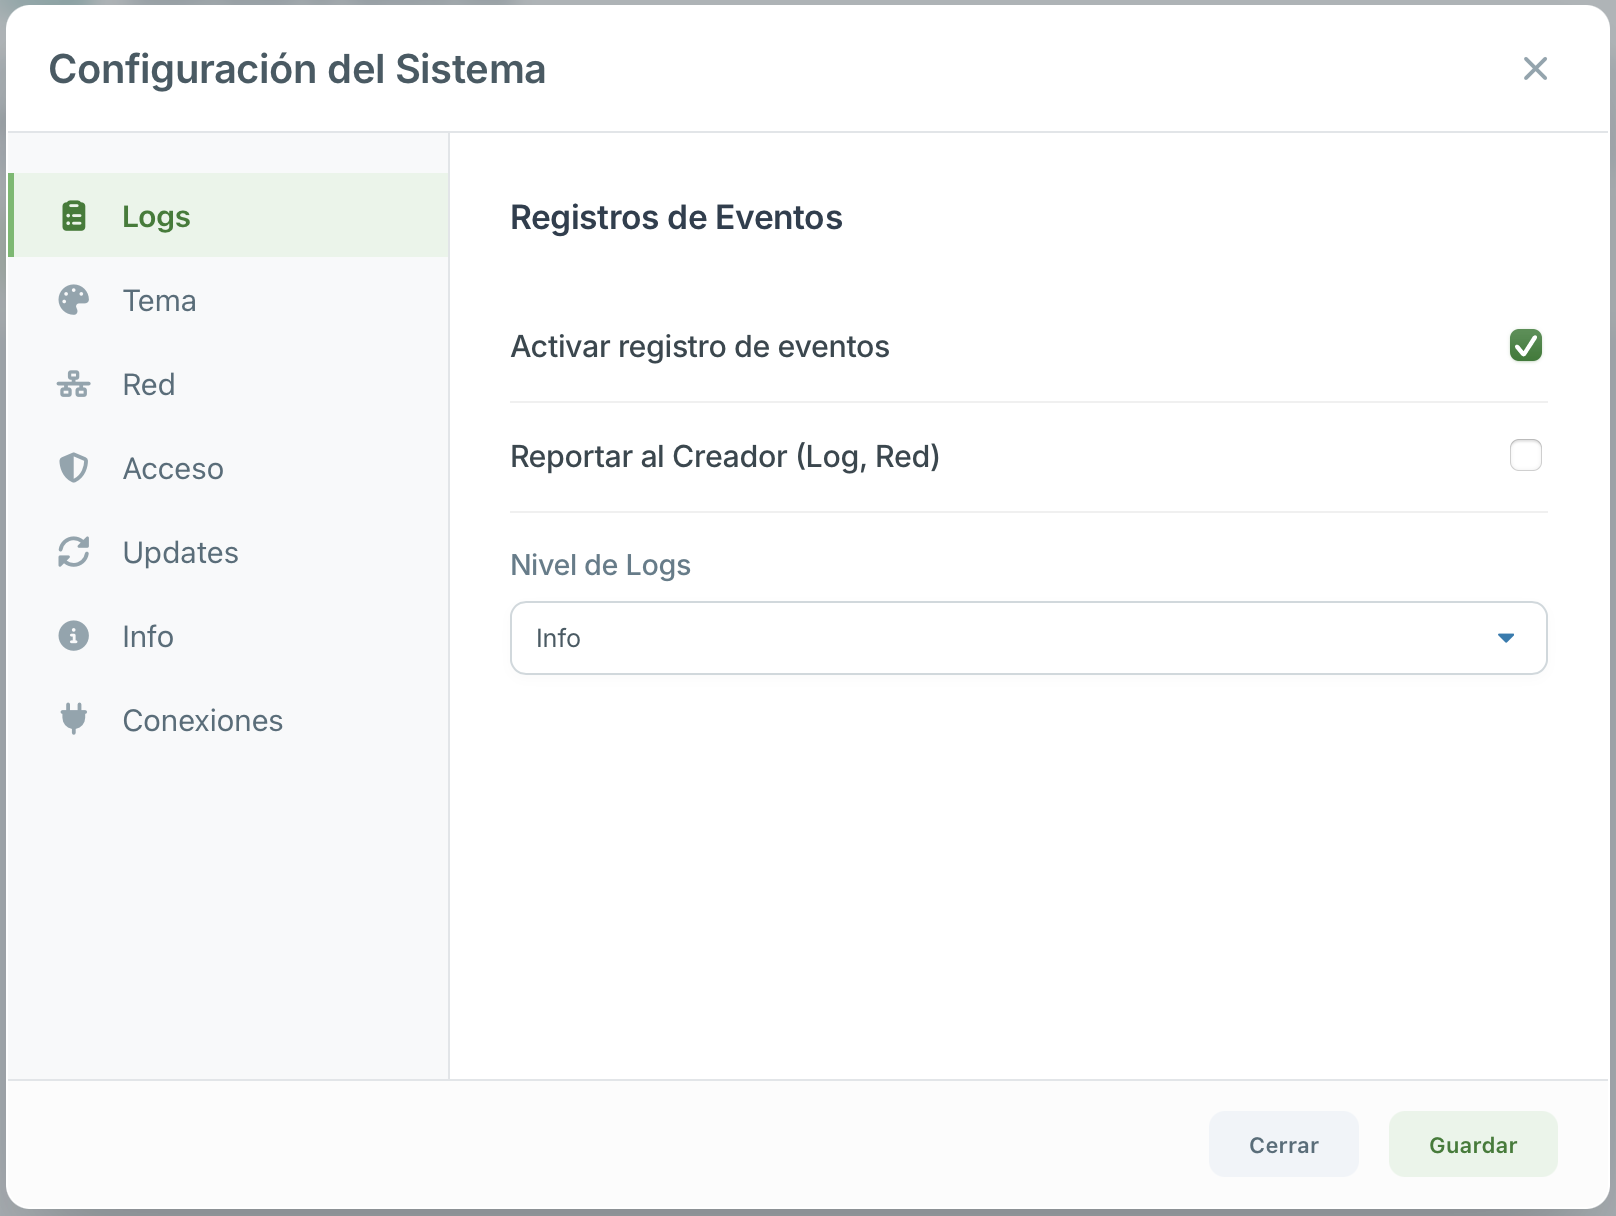
\includegraphics[width=0.95\textwidth]{anexos/15 configurador.png}
\caption{Configurador del visor de documentos}
\label{fig:configurador}
\end{figure}

\subsection{Opciones de Configuracion}

\begin{table}[H]
\centering
\begin{tabular}{p{5cm}p{3cm}p{5cm}}
\toprule
\textbf{Opcion} & \textbf{Valores} & \textbf{Efecto} \\
\midrule
Auto-cierre por inactividad & 1-60 minutos & Cierra documento tras inactividad \\
\midrule
Prevenir capturas de pantalla & Si / No & Bloquea PrintScreen y grabacion \\
\midrule
Marcas de agua dinamicas & Si / No & Superpone ID de sesion en vista \\
\midrule
Nivel de zoom por defecto & 50-200 por ciento & Ajuste inicial de visualizacion \\
\bottomrule
\end{tabular}
\caption{Opciones de configuracion del visor}
\label{tab:config-visor}
\end{table}

\begin{quote}
\textbf{Marcas de Agua Dinamicas}\\
Cuando estan activadas, el visor superpone una marca de agua semitransparente que incluye: Client ID del nodo, timestamp de apertura, y nombre de usuario.
\end{quote}

\section{Flujo de Seguridad del Visor}

El proceso de seguridad del visor sigue estos pasos:

\begin{enumerate}
    \item \textbf{Solicitud de Apertura}: El usuario solicita abrir un documento
    \item \textbf{Autorizacion}: Verificacion de permisos y credenciales
    \item \textbf{Descifrado en RAM}: El documento se descifra en memoria volatil
    \item \textbf{Renderizado}: Visualizacion del contenido descifrado
    \item \textbf{Visualizacion Activa}: El usuario interactua con el documento
    \item \textbf{Cierre}: Al cerrar, se aplica zero-fill a la memoria
    \item \textbf{Registro de Auditoria}: Se registra el evento de acceso
\end{enumerate}

\section{Mejores Practicas}

\begin{enumerate}[leftmargin=*]
    \item Cierra siempre el visor cuando termines de trabajar con documentos sensibles
    \item Habilita el auto-cierre por inactividad (recomendado: 5 minutos)
    \item Usa marcas de agua en entornos compartidos
    \item Bloquea capturas de pantalla para documentos altamente confidenciales
    \item Verifica el hash antes de abrir documentos descargados
\end{enumerate}

\begin{quote}
\textbf{Responsabilidad del Usuario}\\
Aunque el visor proporciona proteccion tecnica robusta, la seguridad final depende del comportamiento del usuario: no fotografiar la pantalla con dispositivos externos, no transcribir informacion sensible a otros medios, cerrar sesion al alejarse del equipo.
\end{quote}
